%%%%%%%%
\subsection{Segmentación de Imágenes}
La segmentación de imágenes es el proceso de dividir una imagen en diferentes partes o regiones, con el objetivo de simplificar la representación de la imagen y hacerla más significativa y fácil de analizar. Este proceso es fundamental en aplicaciones de visión por computadora, especialmente en la detección de características morfológicas de la piel, como arrugas, poros y manchas \cite{autor2020segmentacion}.

\subsection{Características Morfológicas de la Piel}
Las características morfológicas de la piel desempeñan un papel crucial en la evaluación de la salud y la estética facial, ya que ofrecen información valiosa sobre el estado general de la piel y sus posibles alteraciones. En este estudio, se consideran tres características clave: arrugas, poros y manchas. La correcta segmentación de estas características en imágenes faciales permite no solo el análisis cuantitativo de las mismas, sino también su monitoreo a lo largo del tiempo, contribuyendo al diseño de tratamientos cosméticos personalizados y a la evaluación de su efectividad.

\subsubsection{Arrugas}
Las arrugas son pliegues o líneas visibles en la superficie de la piel que se forman debido a la disminución de la elasticidad y el colágeno con el envejecimiento. Factores externos, como la exposición prolongada al sol, la contaminación y el tabaquismo, también contribuyen significativamente a su aparición. Además, las expresiones faciales repetitivas y la deshidratación de la piel pueden acelerar su desarrollo.

Desde el punto de vista estético, las arrugas se asocian con el envejecimiento y son una de las principales preocupaciones en el cuidado de la piel. Su segmentación precisa permite identificar su profundidad, longitud y densidad en diferentes áreas del rostro. Esta información es esencial para el desarrollo de productos antiarrugas y para evaluar la efectividad de tratamientos como cremas tópicas, terapias con láser o inyecciones de ácido hialurónico \cite{autor2021arrugas}.

\subsubsection{Poros}
Los poros son pequeñas aberturas en la piel a través de las cuales las glándulas sebáceas secretan sebo, un aceite natural que mantiene la piel hidratada y protegida. Su tamaño y visibilidad pueden variar según factores como la genética, el tipo de piel y los niveles hormonales. Los poros dilatados son una preocupación común, especialmente en personas con piel grasa, ya que pueden contribuir a la apariencia de una textura desigual y al desarrollo de imperfecciones, como puntos negros o acné.

La segmentación de poros en imágenes faciales proporciona una forma de cuantificar su tamaño, densidad y distribución, permitiendo una evaluación más objetiva. Esto es particularmente útil en estudios sobre tratamientos que buscan reducir su visibilidad, como peelings químicos, productos con retinoides o técnicas de microdermoabrasión \cite{autor2020poros}.

\subsubsection{Manchas}
Las manchas son áreas de hiperpigmentación o hipopigmentación en la piel que resultan de una variedad de factores, incluyendo la exposición solar prolongada, cambios hormonales, envejecimiento y procesos inflamatorios. Ejemplos comunes incluyen el melasma, las manchas solares y las cicatrices post-inflamatorias.

Estas imperfecciones no solo afectan la apariencia de la piel, sino que también pueden indicar daño subyacente. Por ello, su detección y análisis temprano son fundamentales tanto para la prevención como para el tratamiento. La segmentación precisa de manchas en imágenes faciales permite identificar su forma, tamaño, color y evolución, lo que es útil para personalizar tratamientos como cremas despigmentantes, terapias con luz pulsada intensa (IPL) o procedimientos láser. Además, este análisis contribuye al diseño de cosméticos específicos que ayudan a unificar el tono de la piel \cite{autor2019manchas}.
%%%%%%%%%%
\subsection{Redes Neuronales Convolucionales (CNN)}  
Las Redes Neuronales Convolucionales (CNN, por sus siglas en inglés) son un modelo de aprendizaje profundo ampliamente utilizado en tareas relacionadas con el procesamiento de imágenes, debido a su capacidad para extraer y aprender automáticamente características relevantes de los datos visuales. Estas redes se componen de varias capas interconectadas que trabajan de manera jerárquica para identificar patrones, desde los más simples, como bordes o texturas, hasta estructuras más complejas \cite{autor2022cnn}. 

\subsubsection{Estructura de las CNN}  
La arquitectura de una CNN incluye varias capas principales, cada una con un propósito específico:
\begin{itemize}
    \item \textbf{Capa convolucional:} Esta capa aplica filtros o kernels sobre la imagen de entrada para extraer características locales como bordes, esquinas y texturas. Cada filtro actúa como un detector especializado en identificar ciertas características.
    \item \textbf{Capa de pooling:} Reduce la dimensionalidad de los datos al seleccionar los valores más representativos (por ejemplo, el máximo o el promedio) dentro de una región específica. Esto hace que el modelo sea más eficiente y robusto frente a pequeñas variaciones en la posición de las características.
    \item \textbf{Capa de activación:} Introduce no linealidad en la red, permitiendo que la CNN aprenda relaciones complejas entre las características. Una de las funciones más comunes es la ReLU (Rectified Linear Unit), que activa únicamente valores positivos.
    \item \textbf{Capas totalmente conectadas:} Estas capas, ubicadas al final de la red, combinan las características extraídas para realizar tareas específicas, como clasificación o segmentación.
\end{itemize}

\subsubsection{Aplicaciones en Segmentación de Imágenes Faciales}  
En el ámbito del análisis de piel facial, las CNN son una herramienta fundamental para realizar segmentaciones precisas de características morfológicas, como arrugas, poros y manchas. Gracias a su capacidad para analizar imágenes a nivel de píxel, estas redes son capaces de identificar patrones y diferencias en la textura, el color y la estructura de la piel \cite{autor2021deep}.

\paragraph{Segmentación de arrugas.}  
La segmentación de arrugas mediante CNN permite identificar líneas finas y pliegues en la piel, lo que es crucial para evaluar el envejecimiento facial y desarrollar tratamientos preventivos o correctivos. Este análisis automatizado es más preciso y rápido en comparación con las evaluaciones manuales, que pueden ser subjetivas y menos consistentes.

\paragraph{Detección de poros.}  
La identificación y segmentación de poros faciales es esencial para analizar problemas relacionados con la textura de la piel, como poros dilatados o acné. Las CNN pueden cuantificar el tamaño, la densidad y la distribución de los poros, facilitando la personalización de tratamientos según las necesidades específicas de cada individuo.

\paragraph{Segmentación de manchas.}  
Las manchas faciales, que pueden surgir debido a factores como la exposición solar o el envejecimiento, son una preocupación estética común. Las CNN permiten mapear su distribución y evaluar su progresión, ayudando a diagnosticar problemas como el melasma o el daño solar de manera temprana y objetiva \cite{autor2020imagen}.

\subsubsection{Ventajas y Limitaciones}  
Las CNN ofrecen varias ventajas, entre ellas:
\begin{itemize}
    \item Alta precisión en la extracción y análisis de características complejas.
    \item Automatización de procesos que tradicionalmente dependen de evaluaciones subjetivas.
    \item Adaptabilidad a diferentes tipos de imágenes y tareas específicas.
\end{itemize}

Sin embargo, estas redes también presentan desafíos, como la necesidad de grandes volúmenes de datos etiquetados para el entrenamiento, el alto costo computacional y la posibilidad de sobreajuste si no se implementan técnicas adecuadas de regularización.

En el presente estudio, las CNN se utilizarán para desarrollar un sistema avanzado de segmentación de imágenes faciales, optimizado para la detección de arrugas, poros y manchas. Este enfoque busca contribuir al sector cosmético y de belleza, permitiendo una evaluación estética más precisa y la personalización de tratamientos cosméticos.


%%
\subsection{Modelos de Segmentación}  
En el campo del análisis de imágenes médicas y dermatológicas, se han desarrollado diversos modelos de segmentación basados en redes neuronales profundas. Estos modelos permiten realizar segmentaciones precisas y eficientes al analizar características específicas de las imágenes, como arrugas, poros y manchas en la piel. A continuación, se describen las principales arquitecturas utilizadas en este ámbito.

\subsubsection{U-Net}  
U-Net es una arquitectura diseñada específicamente para tareas de segmentación médica. Su estructura en forma de "U" consta de un camino de codificación y un camino de decodificación.  
\begin{itemize}
    \item \textbf{Camino de codificación:} Extrae características importantes de la imagen mediante una serie de capas convolucionales y de pooling, reduciendo progresivamente la resolución.
    \item \textbf{Camino de decodificación:} Reconstruye la imagen segmentada al combinar características extraídas con información de niveles anteriores mediante conexiones de salto (\textit{skip connections}).
\end{itemize}  
U-Net es conocida por su capacidad para segmentar detalles finos y preservar el contexto global de la imagen, lo que la hace ideal para analizar características como poros y manchas en imágenes de piel \cite{autor2020unet}.

\subsubsection{Fully Convolutional Network (FCN)}  
Las Fully Convolutional Networks (FCN) transforman las capas completamente conectadas de una red clásica en capas convolucionales, permitiendo que la red produzca mapas de características de tamaño variable.  
\begin{itemize}
    \item \textbf{Segmentación a nivel de píxel:} Al operar directamente sobre cada píxel de la imagen, las FCN son capaces de realizar segmentaciones precisas en tiempo real.
    \item \textbf{Ventaja principal:} Eliminan la necesidad de redimensionar las imágenes a tamaños fijos, preservando la resolución y los detalles contextuales \cite{autor2019fcn}.
\end{itemize}  
Este enfoque es útil en tareas donde la precisión a nivel de píxel es crítica, como en la segmentación de arrugas y texturas de la piel.

\subsubsection{SegNet}  
SegNet es una arquitectura basada en una estructura de codificación-decodificación que se ha optimizado para la segmentación semántica en tiempo real.  
\begin{itemize}
    \item \textbf{Codificador:} Utiliza capas de convolución y pooling para reducir la dimensionalidad y extraer características importantes.
    \item \textbf{Decodificador:} Reconstruye la segmentación mediante el uso de índices de pooling del codificador, lo que mejora la eficiencia computacional.
\end{itemize}  
SegNet es particularmente adecuado para aplicaciones donde los recursos computacionales son limitados, como en dispositivos móviles utilizados para análisis cosméticos \cite{autor2021segnet}.

\subsubsection{Mask R-CNN}  
Mask R-CNN extiende la arquitectura Faster R-CNN para incluir una rama adicional que genera máscaras binarias a nivel de instancia.  
\begin{itemize}
    \item \textbf{Detección de instancias:} Identifica y segmenta objetos específicos dentro de una imagen, lo que la hace adecuada para segmentar poros o manchas de manera individual.
    \item \textbf{Precisión mejorada:} Combina predicciones de clase, cajas delimitadoras y máscaras segmentadas en un solo modelo \cite{autor2022maskrcnn}.
\end{itemize}  
Gracias a su enfoque basado en instancias, Mask R-CNN es ideal para tareas donde se requiere identificar características específicas en imágenes faciales.

\subsubsection{DeepLab (v3, v3+)}  
DeepLab es una familia de modelos que utiliza convoluciones atrous (también conocidas como convoluciones dilatadas) para expandir el campo receptivo de las capas convolucionales sin aumentar la carga computacional.  
\begin{itemize}
    \item \textbf{Convoluciones atrous:} Permiten capturar características en diferentes escalas, lo que es crucial para segmentar detalles finos como arrugas y texturas complejas de la piel.
    \item \textbf{Módulo ASPP:} DeepLab v3/v3+ incorpora un módulo de agrupación espacial piramidal (\textit{Atrous Spatial Pyramid Pooling}) para capturar información contextual a múltiples escalas \cite{autor2021deeplab}.
    \item \textbf{Versión v3+:} Añade un decodificador para mejorar la segmentación en bordes y detalles, lo que la hace especialmente útil para el análisis dermatológico detallado.
\end{itemize}  

\paragraph{Comparativa de Modelos}  
Cada modelo de segmentación ofrece ventajas particulares dependiendo del contexto:
\begin{itemize}
    \item U-Net y DeepLab son ideales para segmentación de características morfológicas de la piel debido a su precisión en detalles finos.
    \item SegNet y FCN son opciones eficientes para aplicaciones en tiempo real.
    \item Mask R-CNN sobresale en la segmentación de instancias específicas, como manchas aisladas.
\end{itemize}  
En esta investigación, se seleccionará la arquitectura más adecuada en función de los requisitos de precisión, recursos computacionales y características específicas a analizar.
%%%%%%%%%%
\subsection{Métricas de Evaluación}  
Las métricas de evaluación son fundamentales para medir la precisión y eficacia de los modelos de segmentación de imágenes, ya que permiten comparar la segmentación automática generada por el modelo con las segmentaciones de referencia (verdaderas). A continuación se describen las principales métricas utilizadas en este tipo de análisis.

\subsubsection{Índice de Sorensen-Dice (Dice Coefficient)}  
El índice de Sorensen-Dice, o simplemente Dice coefficient, es una métrica ampliamente utilizada para evaluar la similitud entre dos conjuntos de datos segmentados. Esta métrica es especialmente útil en problemas de segmentación de imágenes médicas, donde es necesario comparar la segmentación automática con la segmentación de referencia.  
\begin{itemize}
    \item \textbf{Fórmula:}  
    \[
    \text{Dice} = \frac{2|A \cap B|}{|A| + |B|}
    \]
    donde \( A \) y \( B \) son los conjuntos de píxeles segmentados de la imagen predicha y la imagen real, respectivamente.
    \item \textbf{Interpretación:} El valor de Dice oscila entre 0 y 1, donde 1 indica una coincidencia perfecta entre las dos segmentaciones, y 0 indica ninguna superposición.
    \item \textbf{Aplicación:} Es útil para tareas donde se requiere alta precisión en la identificación de áreas segmentadas, como en el análisis de manchas y arrugas en la piel, donde una segmentación precisa es crucial \cite{autor2020dice}.
\end{itemize}

\subsubsection{Coeficiente de Jaccard (Intersection over Union, IoU)}  
El coeficiente de Jaccard, también conocido como \( \text{Intersection over Union} \) (IoU), es otra métrica popular para evaluar la superposición entre dos conjuntos de segmentación. A diferencia del índice de Dice, IoU mide la relación entre la intersección de los conjuntos de píxeles predichos y reales con respecto a su unión total.  
\begin{itemize}
    \item \textbf{Fórmula:}  
    \[
    \text{IoU} = \frac{|A \cap B|}{|A \cup B|}
    \]
    donde \( A \) y \( B \) son los conjuntos de píxeles segmentados de la imagen predicha y la imagen real, respectivamente.
    \item \textbf{Interpretación:} El valor de IoU también varía entre 0 y 1. Un valor más alto indica una mayor superposición entre los segmentos predichos y reales. IoU es especialmente útil cuando se requiere evaluar la precisión en áreas de segmentación con bordes definidos, como en el análisis de arrugas y poros \cite{autor2021iou}.
    \item \textbf{Aplicación:} Es más severo que el índice de Dice, por lo que es adecuado para evaluar tareas donde la precisión en los bordes y las áreas superpuestas es esencial.
\end{itemize}

\subsubsection{Precisión (Precision)}  
La precisión es una métrica que refleja la efectividad del modelo en evitar falsos positivos. Se calcula como la relación entre los verdaderos positivos y el total de elementos que el modelo ha predicho como positivos. En el contexto de la segmentación de imágenes, la precisión mide la exactitud de las regiones predichas como relevantes por el modelo.  
\begin{itemize}
    \item \textbf{Fórmula:}  
    \[
    \text{Precisión} = \frac{TP}{TP + FP}
    \]
    donde \( TP \) son los verdaderos positivos (píxeles correctamente predichos como parte de la característica) y \( FP \) son los falsos positivos (píxeles incorrectamente predichos como parte de la característica).
    \item \textbf{Interpretación:} Un valor más alto de precisión indica que el modelo es más efectivo en minimizar los falsos positivos, lo cual es crítico en aplicaciones dermatológicas, donde un modelo debe evitar identificar incorrectamente áreas no relevantes como características de la piel.
    \item \textbf{Aplicación:} Es útil para tareas donde el modelo debe ser riguroso en evitar predecir áreas de la imagen que no pertenecen a la característica de interés, como en el caso de la segmentación de manchas o poros \cite{autor2019precision}.
\end{itemize}

\subsubsection{Entropía Cruzada (Cross-Entropy)}  
La entropía cruzada es una función de pérdida utilizada comúnmente en problemas de clasificación y segmentación. Mide la disonancia o la diferencia entre la distribución de probabilidad predicha por el modelo y la distribución de probabilidad real (etiquetas verdaderas). En el contexto de la segmentación, la entropía cruzada es utilizada para entrenar el modelo, ya que penaliza las predicciones incorrectas.  
\begin{itemize}
    \item \textbf{Fórmula:}  
    \[
    \text{Cross-Entropy} = -\sum_{i} y_i \log(p_i)
    \]
    donde \( y_i \) es la etiqueta real de la clase \( i \) y \( p_i \) es la probabilidad predicha para la clase \( i \).
    \item \textbf{Interpretación:} Un valor bajo de entropía cruzada indica que el modelo ha aprendido bien a predecir las clases correctas, es decir, las características de la piel en las imágenes segmentadas. Un valor alto sugiere una mala predicción, lo que indica que el modelo está lejos de la distribución real.
    \item \textbf{Aplicación:} La entropía cruzada es especialmente útil durante el proceso de entrenamiento para ajustar los parámetros del modelo y garantizar que la segmentación final sea lo más precisa posible, especialmente al tratar con características complejas de la piel como manchas o arrugas \cite{autor2022crossentropy}.
\end{itemize}
%%%
\subsection{Redes de Atención}  
Las redes de atención han surgido como una de las principales innovaciones en el campo de la segmentación de imágenes, permitiendo que los modelos se enfoquen de manera más eficiente en las regiones relevantes de una imagen. Este mecanismo resulta especialmente útil cuando se trabaja con imágenes complejas, como las faciales, donde ciertas áreas contienen características importantes para el análisis, pero pueden ser de menor tamaño o estar localizadas en posiciones no centrales.

\subsubsection{Mecanismo de Atención}  
El mecanismo de atención permite a la red asignar diferentes pesos a distintas partes de la imagen durante el proceso de segmentación. Este mecanismo es esencial para que el modelo pueda enfocarse en las áreas relevantes de la imagen, como arrugas, manchas o poros, sin perder detalles importantes de otras zonas. El concepto básico detrás de la atención es que no todas las partes de la imagen son igualmente importantes para la tarea en cuestión. Por lo tanto, la atención ayuda a los modelos a priorizar las áreas clave que impactan en el resultado final.  
\begin{itemize}
    \item \textbf{Funcionamiento:} La atención se puede aplicar de manera global o local. En el caso de la segmentación de imágenes faciales, por ejemplo, el modelo puede aprender a dar más importancia a las áreas alrededor de los ojos o la frente, donde las arrugas suelen ser más notorias.
    \item \textbf{Beneficio:} Aumenta la precisión de la segmentación al concentrarse solo en las características más relevantes y minimizar el "ruido" de otras regiones no significativas \cite{autor2021atencion}.
\end{itemize}

\subsubsection{Atención Espacial}  
La atención espacial es un tipo específico de atención que asigna pesos según la ubicación espacial de los elementos dentro de la imagen. Esto permite al modelo resaltar áreas específicas de la imagen que contienen características clave para la segmentación.  
\begin{itemize}
    \item \textbf{Funcionamiento:} A través de la atención espacial, el modelo puede identificar patrones en las posiciones de las características de interés, como las arrugas en la zona de la frente o las manchas en la mejilla. Este enfoque es útil cuando las características relevantes están distribuidas de manera no uniforme en la imagen.
    \item \textbf{Aplicación:} Es particularmente eficaz en la segmentación de imágenes faciales, donde las características que deben segmentarse no están siempre en el mismo lugar de la imagen y varían según la persona y la expresión facial \cite{autor2020spa}.
\end{itemize}

\subsubsection{Atención de Canal}  
La atención de canal se enfoca en las características dentro de los canales de la imagen, es decir, en las distintas representaciones de las características de la imagen que corresponden a las diferentes profundidades o colores de los filtros en una red convolucional. Este tipo de atención permite que la red enfoque su procesamiento en los canales que contienen la información más relevante para la tarea.  
\begin{itemize}
    \item \textbf{Funcionamiento:} En lugar de distribuir el enfoque en toda la imagen, la atención de canal resalta los canales específicos que contienen detalles cruciales, como la textura de la piel o las sombras que definen arrugas o manchas.
    \item \textbf{Beneficio:} Mejora la capacidad del modelo para diferenciar entre características de diferentes intensidades o patrones, lo cual es esencial en imágenes donde la variabilidad de la textura de la piel puede ser un desafío \cite{autor2019canal}.
\end{itemize}

\subsubsection{Beneficios de las Redes de Atención}  
Las redes de atención proporcionan varios beneficios clave que mejoran la precisión y eficiencia de los modelos de segmentación, especialmente cuando se trabaja con imágenes complejas como las faciales:
\begin{itemize}
    \item \textbf{Precisión mejorada:} Al permitir que el modelo se enfoque en las regiones más importantes de la imagen, las redes de atención ayudan a obtener segmentaciones más precisas y detalladas.
    \item \textbf{Eficiencia en el procesamiento:} Reduciendo el "ruido" o la información irrelevante, las redes de atención aumentan la eficiencia computacional, ya que el modelo dedica más recursos a las áreas clave.
    \item \textbf{Versatilidad:} Las redes de atención se pueden combinar con otros modelos de segmentación, como U-Net o Mask R-CNN, para mejorar aún más la capacidad del modelo para realizar segmentaciones de alta calidad \cite{autor2021beneficios}.
\end{itemize}

\subsubsection{Ejemplos de Modelos con Atención}  
Existen varios modelos que implementan mecanismos de atención para mejorar la segmentación de imágenes. Algunos ejemplos notables incluyen:
\begin{itemize}
    \item \textbf{Transformer:} El modelo Transformer ha sido exitoso en tareas de procesamiento de secuencias y también ha demostrado ser útil para segmentación de imágenes, particularmente al aplicar atención a nivel global en la imagen. Este modelo asigna pesos no solo localmente, sino también a nivel global, lo que mejora la precisión en tareas complejas de segmentación \cite{autor2022transformer}.
    \item \textbf{SENet:} SENet es una arquitectura que utiliza un módulo de atención de canal para asignar diferentes importancias a los canales de características en una red convolucional. Este modelo ha demostrado ser eficaz en tareas de clasificación y segmentación, particularmente en la mejora de la detección de características sutiles, como pequeñas arrugas o manchas \cite{autor2022senet}.
\end{itemize}

\subsection{Redes Generativas Adversariales (GANs)}  
Las Redes Generativas Adversariales (GANs) son una clase de redes neuronales que consisten en dos submodelos: un generador y un discriminador, que compiten entre sí para mejorar la calidad de los resultados generados. Las GANs han demostrado ser altamente efectivas en la generación de imágenes realistas y en tareas de segmentación, especialmente cuando los datos disponibles son limitados.

\subsubsection{Estructura de GANs (Generador y Discriminador)}  
La estructura básica de las GANs consiste en dos redes que tienen objetivos contrapuestos:
\begin{itemize}
    \item \textbf{Generador:} El generador crea datos falsos a partir de ruido aleatorio o datos incompletos, tratando de producir imágenes que sean indistinguibles de las reales.
    \item \textbf{Discriminador:} El discriminador tiene la tarea de clasificar las imágenes generadas como reales o falsas, evaluando su autenticidad.
\end{itemize}
A lo largo del proceso de entrenamiento, el generador intenta engañar al discriminador para que clasifique sus imágenes como reales, mientras que el discriminador mejora en la detección de imágenes falsas. Este proceso de competencia mejora gradualmente la calidad de las imágenes generadas.  
\begin{itemize}
    \item \textbf{Aplicación en Segmentación:} Las GANs se utilizan en la segmentación de imágenes cuando se dispone de un conjunto de datos limitado, ya que el generador puede crear imágenes realistas que amplían el conjunto de entrenamiento y ayudan a mejorar la capacidad del modelo de segmentación \cite{autor2020gans}.
\end{itemize}

\subsubsection{Aplicaciones de GANs en Segmentación}  
Las GANs se han utilizado con éxito en diversas aplicaciones de segmentación, especialmente cuando se enfrenta a desafíos como conjuntos de datos pequeños o imágenes ruidosas. Algunas de sus aplicaciones incluyen:
\begin{itemize}
    \item \textbf{Generación de datos sintéticos:} En áreas como la dermatología, donde puede ser difícil obtener grandes volúmenes de imágenes etiquetadas, las GANs pueden generar imágenes sintéticas que representan diversas condiciones de la piel, lo que amplía el conjunto de datos de entrenamiento.
    \item \textbf{Segmentación de imágenes:} Las GANs también se aplican directamente a la segmentación de imágenes, especialmente en la mejora de la precisión en bordes complejos, como los que definen arrugas o manchas, a través de la generación de nuevas muestras \cite{autor2021gans_segmentacion}.
\end{itemize}

\subsubsection{Variantes de GANs (CycleGAN, Pix2Pix)}  
Existen variantes de las GANs que mejoran la capacidad de las redes para realizar tareas de segmentación de manera más efectiva:
\begin{itemize}
    \item \textbf{CycleGAN:} CycleGAN es una variante que se utiliza para la traducción de imágenes entre dominios, es decir, transformar imágenes de un estilo a otro, como convertir imágenes de baja resolución a alta resolución o generar imágenes en diferentes condiciones de iluminación. Este modelo puede ser útil en segmentación cuando las imágenes de entrada varían significativamente entre diferentes dominios \cite{autor2019cyclegan}.
    \item \textbf{Pix2Pix:} Pix2Pix es otro modelo basado en GAN que se usa para la segmentación supervisada, donde el modelo aprende a mapear una imagen de entrada a una imagen de salida. Se ha aplicado exitosamente en tareas de segmentación de imágenes faciales y dermatológicas, donde se requiere una alta precisión en los bordes de las características segmentadas \cite{autor2019pix2pix}.
\end{itemize}

\subsubsection{Desafíos de las GANs}  
A pesar de su éxito, las GANs enfrentan varios desafíos importantes:
\begin{itemize}
    \item \textbf{Inestabilidad en el entrenamiento:} Durante el entrenamiento, el generador y el discriminador pueden no converger correctamente, lo que puede llevar a resultados inconsistentes o de baja calidad.
    \item \textbf{Modo colapso:} Un desafío común en las GANs es el "modo colapso", donde el generador produce una variedad limitada de muestras, afectando la diversidad de los datos generados. Este problema puede resultar en segmentaciones menos precisas o en la falta de variabilidad en las características segmentadas \cite{autor2022challenges_gans}.
\end{itemize}


\begin{comment}

\subsection{Ecografía y las imágenes de ultrasonido}
Según \cite{pr_herrera2017diseimp}, la ecografía, que es una técnica de diagnóstico en donde se usan imágenes generadas por ultrasonido, es comúnmente desarrollado en las áreas de cardiología, ginecología, y otras más relacionadas. La popularidad de esta técnica se basa en la capacidad de las imágenes de alta calidad que se obtienen de este proceso, además de no ser un método invasivo o de radiación como muchos otros de su tipo.

Los sistema encargados de extraer las imágenes de ultrasonido son compuestos de distintas sensores que generan ondas de sonido para posteriormente analizar la respuesta de la interacción física con el campo de interés. Estas señales recibidas de regreso son digitalizados por una parte electrónica delantera que también transforman estos datos crudos en la imagen final. El funcionamiento de este proceso depende de la configuración de los sensores, el método usado para obtener las imágenes y las características de área de interés. \parencite{pr_camacho2022ultrasonicimg}

Algunas imágenes de ultrasonido de nódulos tiroideos se muestran en la Figura \ref{2:fig210}.

\begin{figure}[H]
	\begin{center}
		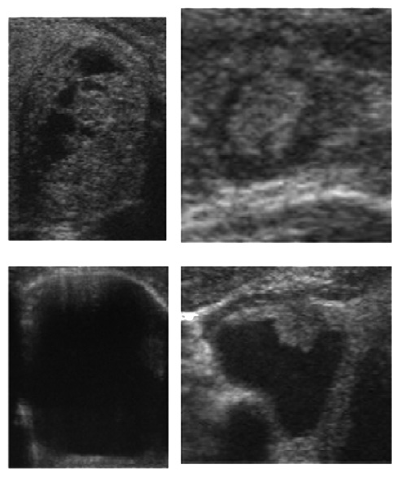
\includegraphics[width=0.40\textwidth]{2/figures/imagenes_ultrasonido_originales.png}
		\caption[Imágenes de ultrasonido de nódulos tiroideos]{Imágenes de ultrasonido de nódulos tiroideos. \\
		Fuente: \cite{pr_JERBI2023autoclassViTGAN}. \textit{Automatic classification of ultrasound thyroids images using vision transformers and generative adversarial networks}.}
		\label{2:fig210}
	\end{center}
\end{figure}


\subsection{Transfer Learning}
\cite{bk_geron2022handml} nos menciona que el Transfer Learning o Transferencia de Aprendizaje es un técnica usada en el campo de Deep Learning que permite el uso de algunas capas de un modelo ya definido y entrenado previamente en un nuevo modelo que necesite ser entrenado en una tarea similar al que se desarrolla el modelo original. Las capas destinadas al reuso son normalmente las más cercanas a la entrada o también conocidas como capas inferiores. El beneficio de usar esta técnica radica en dos puntos importantes: cantidad de datos requeridos y velocidad de entrenamiento del modelo; es decir, la cantidad de datos que se deben usar para entrenar un modelo de alto desempeño se reduce considerablemente, mientras que el tiempo requerido para terminar este proceso es menor comparándolo a si lo entrenaran desde cero.

Para que esta técnica funcione debidamente, las capas más cercanas a la salida, conocidas también como capas de alto nivel, deben ser reemplazadas, esto debido a que son más específicas de las tareas del modelo original. Esto también incluye a la capa final, ya que posiblemente no tenga la cantidad de salidas necesarias para completar satisfactoriamente la nueva tarea.

En la Figura \ref{2:fig211} se presenta de forma gráfica la técnica.

\begin{figure}[H]
	\begin{center}
		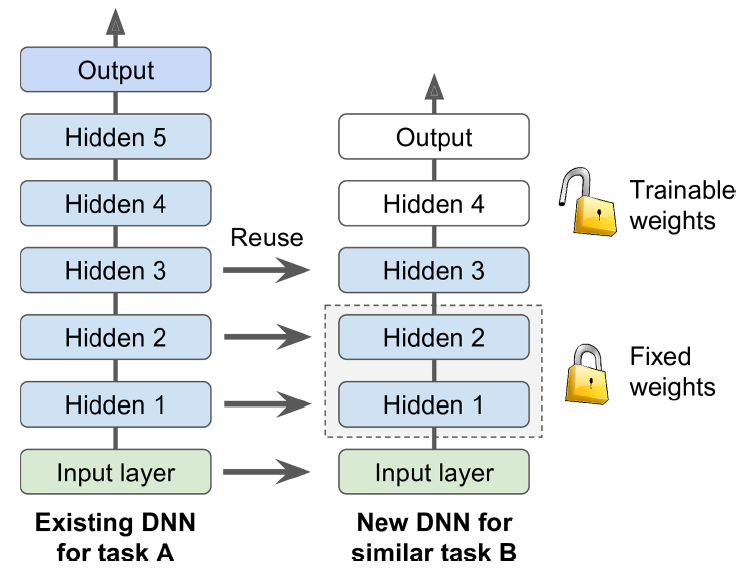
\includegraphics[width=0.70\textwidth]{2/figures/transfer_learning.PNG}
		\caption[Ejemplo de Transfer Learning]{Ejemplo de Transfer Learning. \\
		Fuente: \cite{bk_geron2022handml}. \textit{Hands-on machine learning with Scikit-Learn, Keras, and TensorFlow}.}
		\label{2:fig211}
	\end{center}
\end{figure}


\subsection{Data Augmentation}

Según \cite{bk_geron2022handml} el Aumento de Datos o Data Augmentation es una técnica de regularización que permite reforzar la cantidad de muestras en un conjunto de datos. Esto se realiza a través de la generación de nuevas instancias similares a los originales; es decir, las personas no deberían ser capaces de diferenciar una imagen generada de una del propio conjunto de datos.

Para generar estas nuevas muestras, normalmente se aplican diferentes transformaciones a las instancias del conjunto de datos original. Estas transformaciones pueden ser; por ejemplo, una simple rotación o recorte de la imagen, siempre y cuando no altere por completo su sentido como es el caso de voltear una imagen de texto de forma horizontal. 

El principal beneficio de esta técnica es que permite reducir el sobreajuste de los modelos entrenados. 

En la Figura \ref{2:fig212} se muestran algunas transformaciones que se pueden hacer al aplicar el Aumento de Datos. 

\begin{figure}[H]
	\begin{center}
		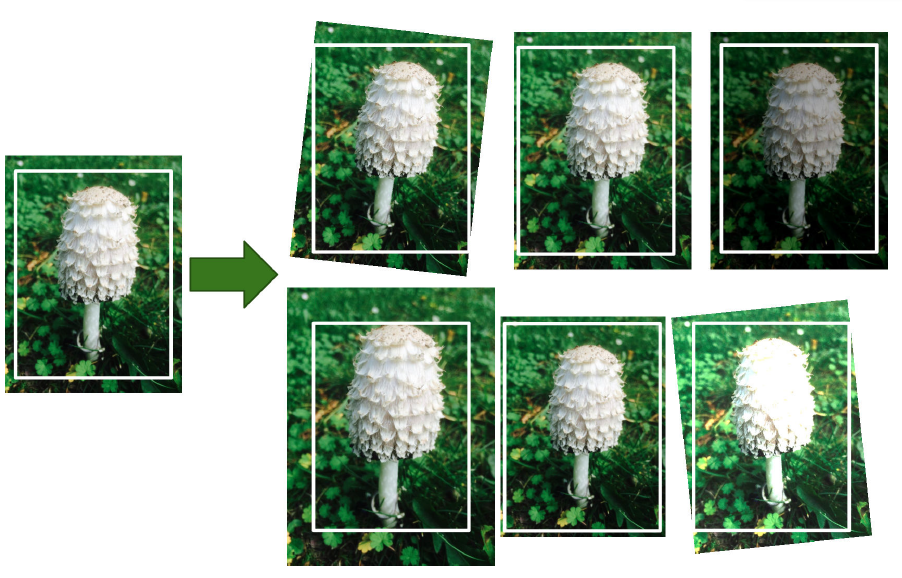
\includegraphics[width=0.85\textwidth]{2/figures/data_aug.PNG}
		\caption[Ejemplo de Data Augmentation]{Ejemplo de Data Augmentation. \\
		Fuente: \cite{bk_geron2022handml}. \textit{Hands-on machine learning with Scikit-Learn, Keras, and TensorFlow}.}
		\label{2:fig212}
	\end{center}
\end{figure}

\end{comment}